\chapter{ Gestionnaire de paquets : \textsc{Kraken}s}
\minitoc
\clearpage

\label{sec:pkgmgr}

\section{Introduction}
\label{sec:intro}

Pour résoudre les limitations de compilation , nous avons mis en place un ensemble d'outils, de scripts et de mécanismes dédiés à la gestion des paquets.  
Cela inclut :
\begin{itemize}
    \item Une structure de dépôt simple ;
    \item Un format de fichier \texttt{PKGBUILD.kraken} pour décrire les paquets ;
    \item Des outils CLI personnalisés pour installer, mettre à jour, supprimer ou rechercher des paquets ;
    \item Un système de gestion des dépendances ;
    \item Un mécanisme de suivi des métadonnées des paquets ;
\end{itemize}

\subsubsection*{Langages s utilisés:}
\begin{figure}[hbt!]
  \centering
  \begin{minipage}[b]{0.18\textwidth}
    
\includegraphics[width=\textwidth]{images_pfe/c.png}
    \caption{C}
  \end{minipage}\hfill
  \begin{minipage}[b]{0.18\textwidth}
    
\includegraphics[width=\textwidth]{images_pfe/bash.jpeg}
    \caption{BASH SCRIPT}
  \end{minipage}\hfill
  \begin{minipage}[b]{0.18\textwidth}
    
\includegraphics[width=\textwidth]{images_pfe/yml.png}
    \caption{YAML}
  \end{minipage}\hfill
  \begin{minipage}[b]{0.18\textwidth}
    
\includegraphics[width=\textwidth]{images_pfe/sqlite.jpeg}
    \caption{SQLITE3}
  \end{minipage}\hfill
  
  \caption{Stack technique de la gestionnaire des paquetes}
  \label{fig:KPGlanguage}
\end{figure}
\FloatBarrier












Notre gestionnaire de paquets se compose de deux composants principaux :
\begin{enumerate}
    \item Le dépôt où sont stockées les métadonnées des paquets ;
    \item Les outils du gestionnaire interagissant avec ce dépôt.
\end{enumerate}

\section{Le dépôt \textsc{Kraken}}
\label{subsec:depot-kraken}

Le dépôt \textsc{Kraken} contient les métadonnées de tous les paquets disponibles, stockées dans des fichiers \texttt{PKGBUILD.kraken}. Chaque fichier décrit la procédure de compilation d'un paquet à partir des sources.

\subsection{Structure du dépôt }
\label{subsubsec:structure-depot}

La structure du dépôt \textsc{Kraken} est conçue pour être lisible, modulaire et maintenable. Chaque paquet correspond à un dossier contenant un fichier \texttt{PKGBUILD.kraken}.\\



\begin{figure}[H]
  \centering
  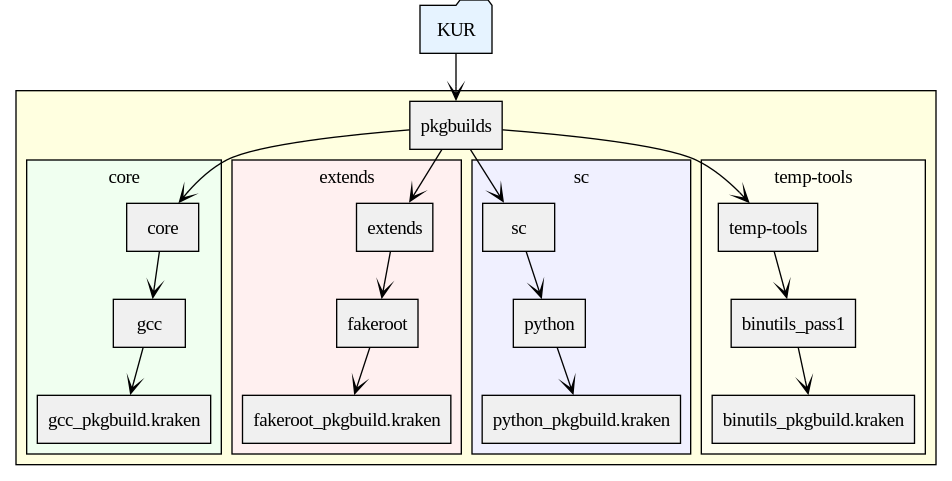
\includegraphics[width=1\textwidth]{images_pfe/repodotoff.png}
  \caption{Structure du dépôt du gestionnaire de paquets \textsc{Kraken}}
  \label{fig:krakenrepo}
\end{figure}

Le dépôt comporte quatre catégories principales :
\begin{itemize}
    \item \textbf{core} : Contient les paquets fondamentaux (gcc, binutils, coreutils...) ;
    \item \textbf{extend} : Paquets d'extension pour enrichir le système (xorg, fakroot, strace...) ;
    \item \textbf{sc} : Outils pour l'informatique (applications web, outils mobiles...) ;
    \item \textbf{temps\_tools} : Outils temporaires pour la chaîne de compilation croisée.
\end{itemize}

\textbf{Note} : Des autre catégories comme  \textbf{math} et \textbf{phys} existent également mais ont été omises pour simplifier la figure.

Chaque paquet dans ces répertoires est décrit par un fichier \texttt{PKGBUILD.kraken} spécifiant sa procédure de construction.

\subsection{Le fichier \texttt{PKGBUILD.kraken}}
\label{subsubsec:pkgbuild-file}

Le fichier \texttt{PKGBUILD.kraken} est un modèle déclaratif décrivant :
\begin{itemize}
    \item La méthode de construction du paquet ;
    \item Ses dépendances ;
    \item Son processus d'installation.
\end{itemize}

\begin{figure}[H]
  \centering
  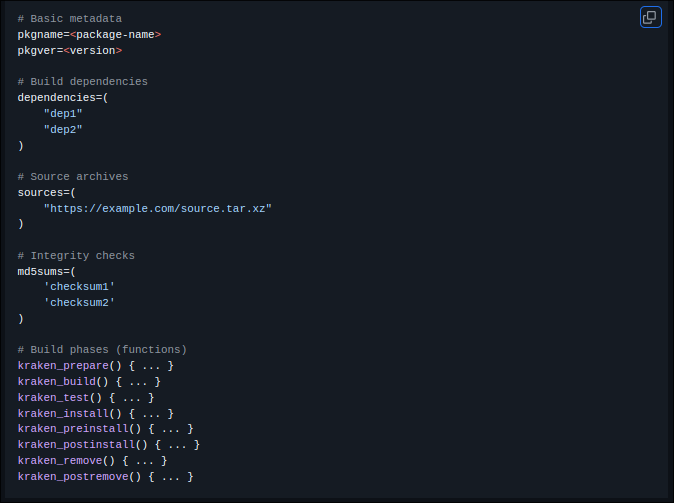
\includegraphics[width=1\textwidth, height=10cm]{images_pfe/pkgbuildkrakenmodle.png}
  \caption{Modèle générique de \texttt{PKGBUILD.kraken}}
  \label{fig:pkgtemplate}
\end{figure}
\clearpage
Exemple concret de \texttt{PKGBUILD.KRAKEN} pour le paquette \texttt{gcc } :
\begin{figure}[H]
  \centering
  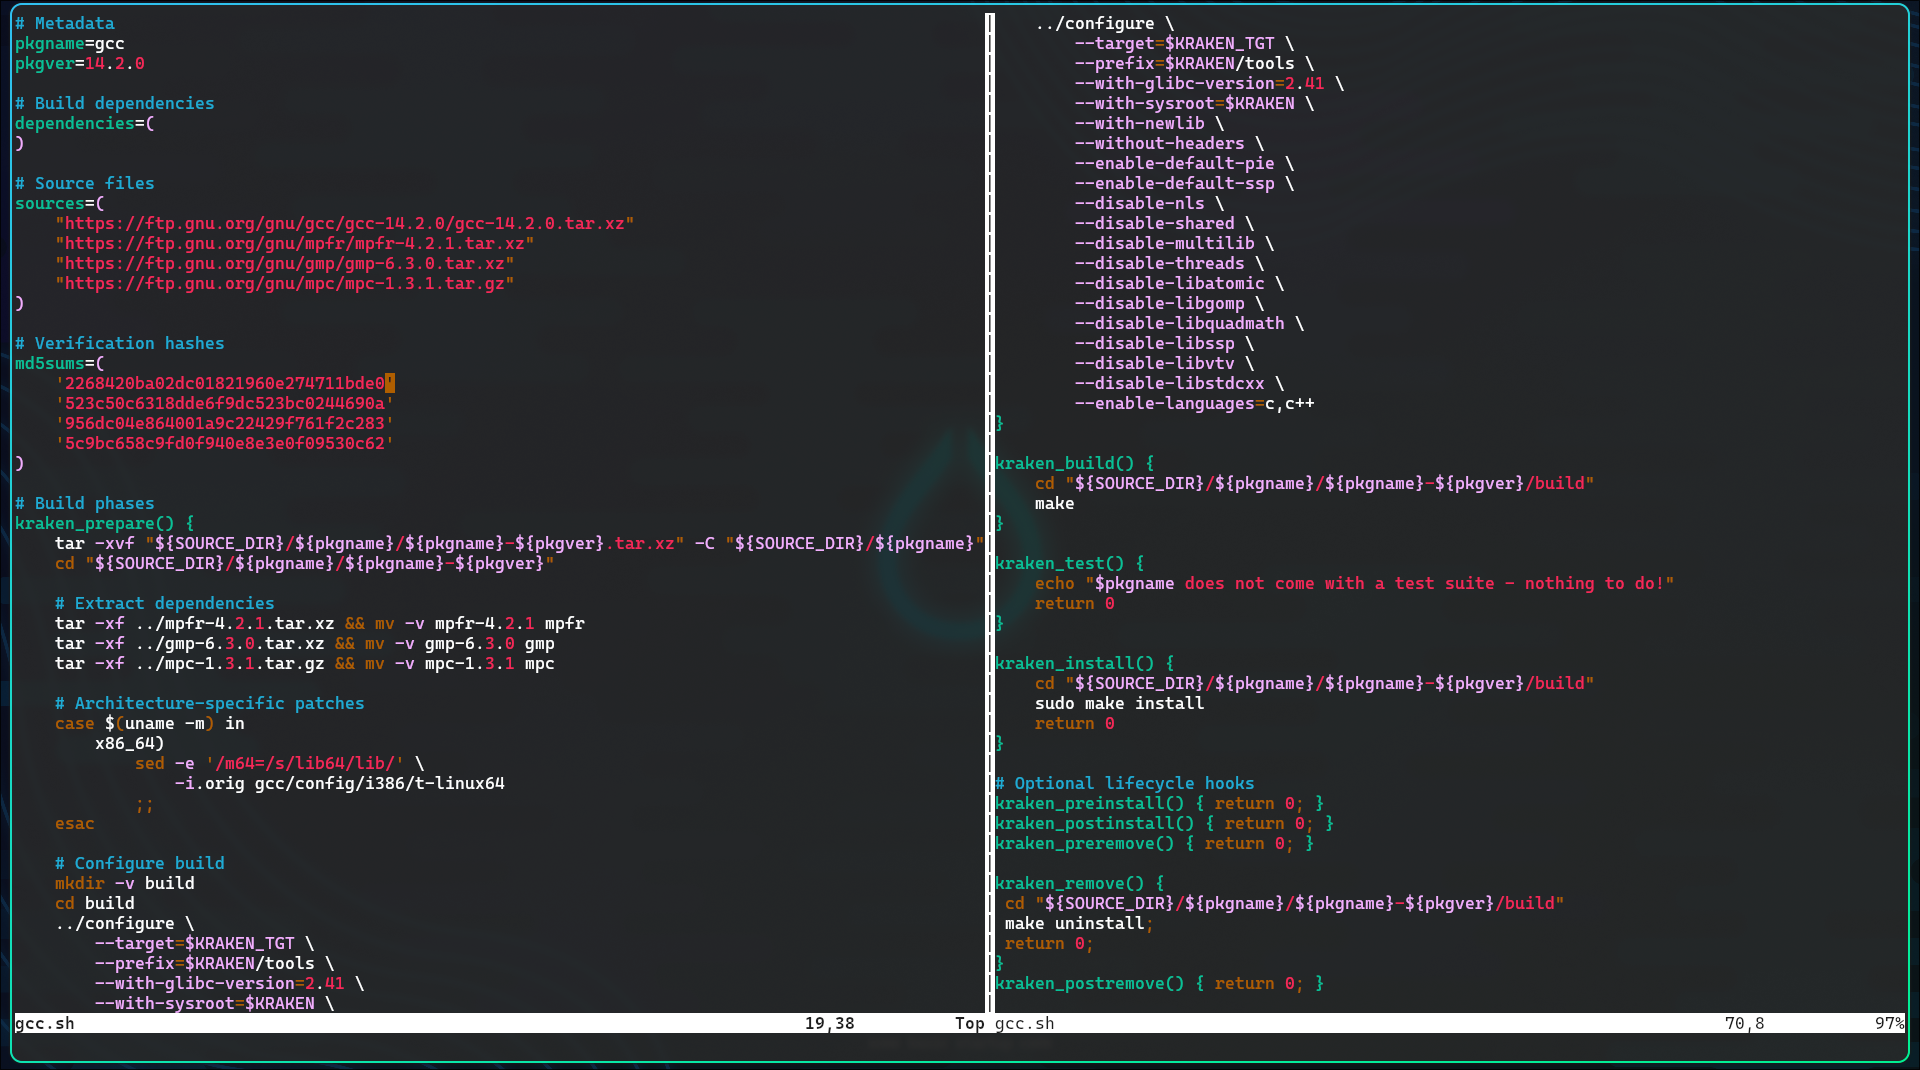
\includegraphics[width=1\textwidth, height=10cm]{images_pfe/exemplepgkbuldgcc.png}
  \caption{Exemple de \texttt{PKGBUILD.kraken} pour le paquet \texttt{gcc}}
  \label{fig:pkgbuildgcc}
\end{figure}

Principales sections du fichier :
\begin{itemize}
    \item \textbf{pkgname}, \textbf{pkgver} : Nom et Version  du paquet ;
    \item \textbf{dependencies} : Dépendances requises avant installation ;
    \item \textbf{sources} : lien de téléchargement de l'archive ;
    \item \textbf{md5sums} : Vérification d'intégrité de l'archive ;
    \item \textbf{kraken-prepare()} : Préparation (extraction, configuration) ;
    \item \textbf{kraken-build()} : Compilation du paquet ;
    \item \textbf{kraken-test} : Procédure de test ;
    \item \textbf{kraken-preinstall} : Préconfigurations avant installation ;
    \item \textbf{kraken-install()} : Installation des fichiers système ;
    \item \textbf{kraken-postinstall} : Postconfigurations (documentation, fichiers) ;
    \item \textbf{kraken-remove} : Procédure de désinstallation.
\end{itemize}

\subsection{Le fichier pkgindex.kraken}
\label{subsubsec:pkgindex}
Le fichier \texttt{pkgindex.kraken} est un index centralisé au format YAML qui contient les métadonnées essentielles de tous les paquets disponibles.
\begin{figure}[H]
  \centering
  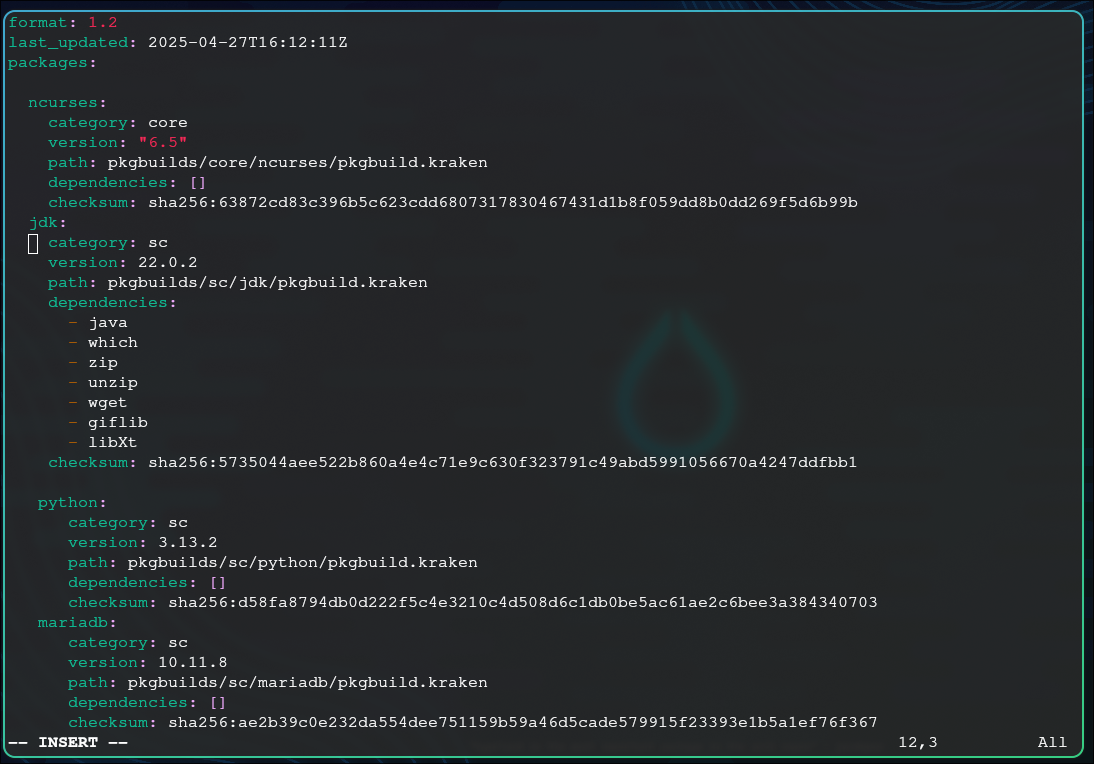
\includegraphics[width=1\textwidth]{images_pfe/pkgindekrakenpkgindex.png}
  \caption{Exemple de fichier pkgindex.kraken}
  \label{fig:pkgindex-example}
\end{figure}

Chaque entrée de paquet contient les champs suivants :
\begin{itemize}
    \item \textbf{category} : Classification fonctionnelle (core, math, physics, etc.)
    \item \textbf{version} : Version de paquets
    \item \textbf{path} : Chemin relatif vers le fichier \texttt{pkgbuild.kraken} dans le depot.
    \item \textbf{dependencies} : Liste des dépendances obligatoires de ce paquetes
    \item \textbf{checksum} : Vérification d'intégrité  du fichier de \texttt{pkgbuild.kraken} de cette paquetes
\end{itemize}
Ce fichier \textbf{généré automatiquement} optimise la recherche de paquets via :
\begin{itemize}
\item \textbf{Réduction} de la complexité de recherche des paquetes dans le depot  de O(n) à O(1) ;
\item \textbf{Mise à jour} instantanée lors des modifications du dépôt ;
\item \textbf{Accès} hors ligne aux métadonnées (versions, dépendances).
\end{itemize}





\clearpage
\subsection{Résumé de la structure du dépôt}
\label{subsec:resume-depot}

Pour résumer cette section :

\begin{itemize}
    \item Le dépôt est organisé en \textbf{répertoires thématiques} classés par domaine (core, extends, sc, math , phys,etc.) ;
    \item Chaque répertoire contient des paquets spécifiques à son domaine ;
    \item Chaque paquet est décrit par un fichier \texttt{PKGBUILD.kraken} qui :
    \begin{itemize}
        \item Est utilise par le gestionnaire de paquets
        \item Contient les instructions de compilation/installation de cette paquette
    \end{itemize}
    \item Le fichier \texttt{pkgindex.kraken} centralise les métadonnées :
    \begin{itemize}
        \item Noms et versions des paquets
        \item Dépendances entre paquets
       \item \textbf{Liens directs} vers les fichiers pkgbuild.kraken de chaque paquet qui existe dans le dépôt.

        \item Permet une recherche optimisée (complexité O(1)) dans le depot.
    \end{itemize}
\end{itemize}





\textcolor{blue}{Code source de la depot (KUR:kraken users repository) disponible dans  \cite{depot_kur}}.
\section{Les outils \textsc{Kraken}}
\label{subsec:kraken-tools}


\




%-------- kraken tools ------------------







Dans cette section, nous présentons les outils en ligne de commande développés pour gérer les paquets à travers le gestionnaire \textsc{Kraken}. Chaque outil est conçu pour exécuter une étape spécifique du cycle de vie d’un paquet : téléchargement, préparation, compilation, test, etc.


\subsection{kraken help}
\label{subsec:kraken-help}

Cet outil fournit à l'utilisateur un menu d'aide comprenant :
\begin{itemize}
    \item La liste des commandes disponibles
    \item Les paramètres acceptés par chaque commande
    \item Des exemples de workflows d'utilisation

\end{itemize}

\begin{figure}[H]
  \centering
  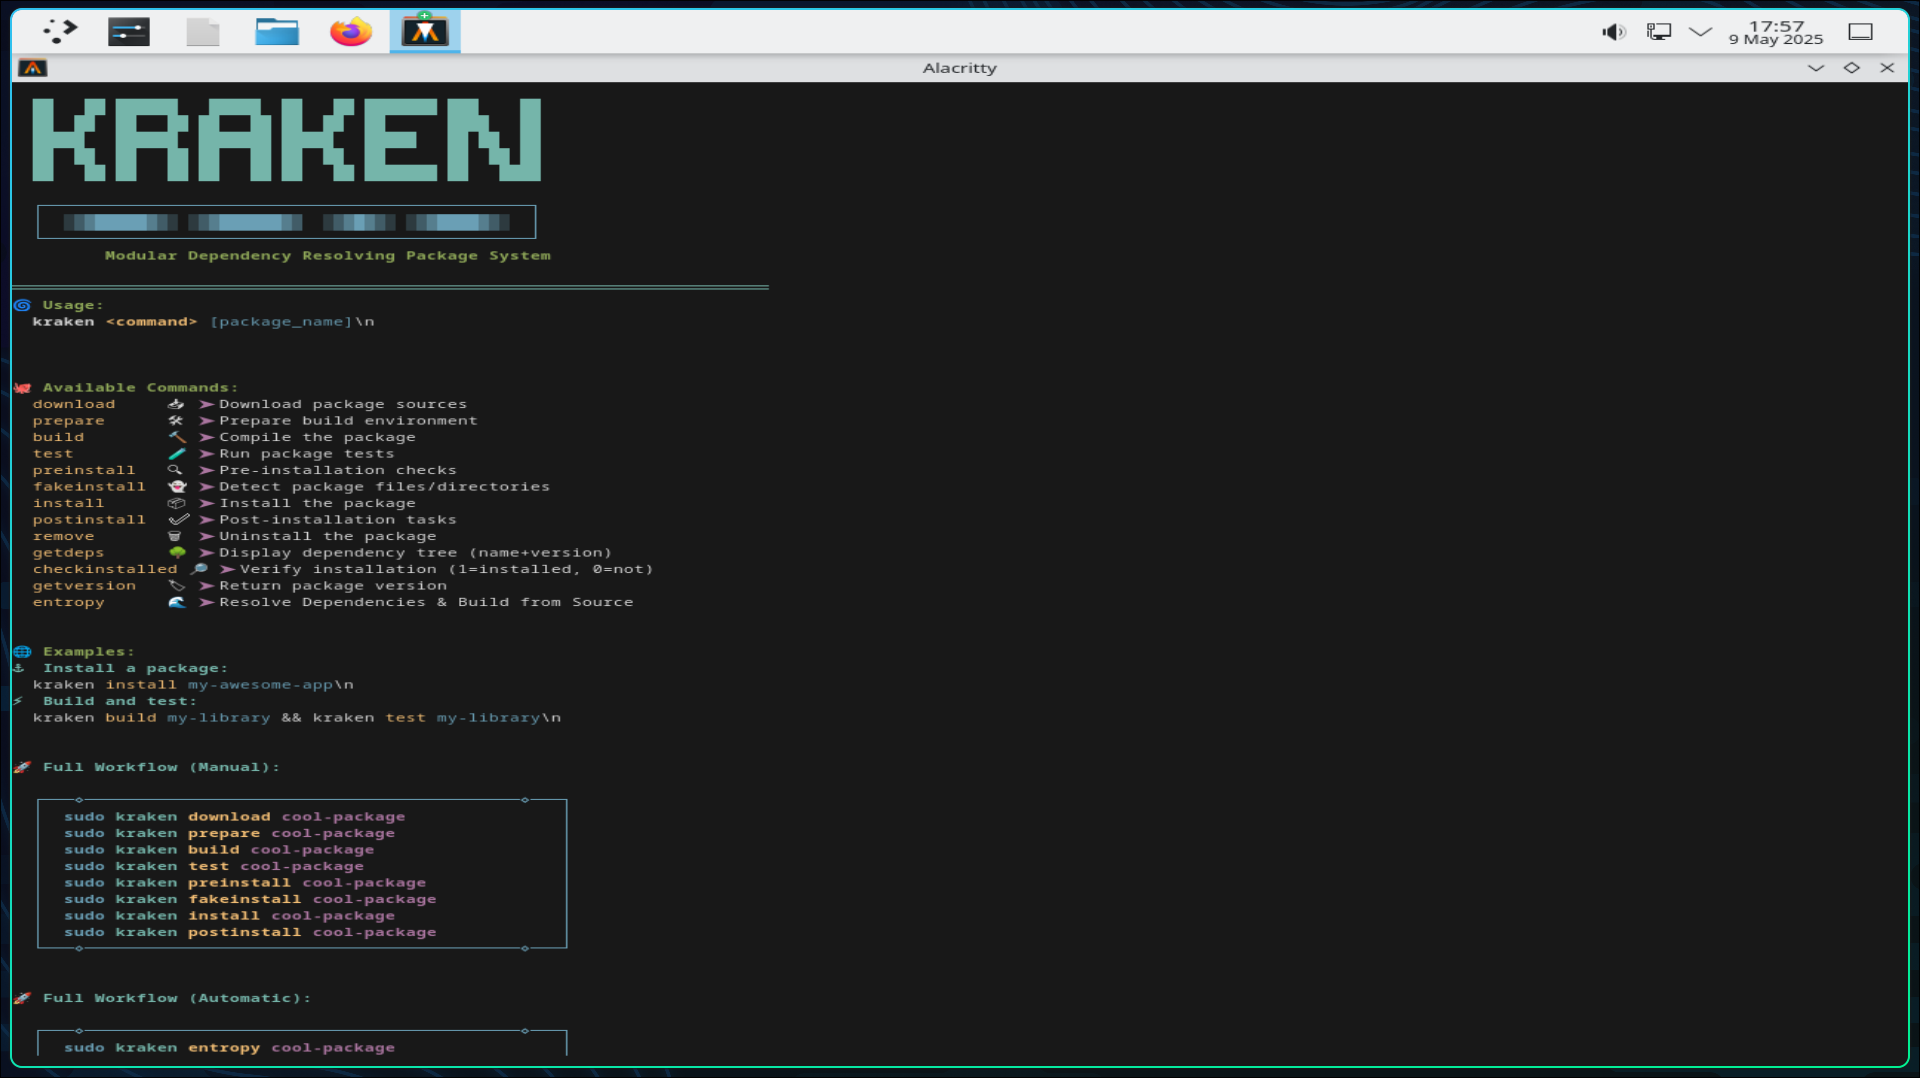
\includegraphics[width=1\textwidth, height=12cm]{images_pfe/krakenhelpmenu.png}
  \caption{Menu d'aide du gestionnaire de paquets \textsc{Kraken}}
  \label{fig:kraken-help}
\end{figure} 

\subsection{kraken download}

\textbf{Utilisation :} \texttt{sudo kraken download <nom\_du\_paquet>}

Cet outil permet de télécharger l’archive (tarball) d’un paquet et de vérifier son intégrité (via \texttt{md5sum}).

\paragraph{Étapes de fonctionnement :}
\begin{enumerate}
    \item Télécharger ou mettre à jour le fichier \texttt{pkgindex.kraken}, et le stocker dans .cache/kraken/krakenindex
    \item Vérifier que le nom du paquet fourni par l'utilisateur existe dans le dépôt depuit le fichier pkgindex.kraken.
    \item Si le paquet existe, créer un répertoire de compilation nommé \texttt{source/}, puis créer un sous-dossier nommé selon le paquet. Dans ce dossier, télécharger le fichier \texttt{PKGBUILD.kraken} et télécharger l’archive du paquet via le champ sources de la ficher pkgbuild.kraken.
    \item Vérifier l'intégrité du fichier \texttt{PKGBUILD.kraken} ainsi que celle de l’archive téléchargée.
    \item Mettre à jour la base de données \texttt{/var/lib/kraken/kraken.db} en marquant le paquet comme téléchargé.
\end{enumerate}

%\begin{figure}[H]
 % \centering
  %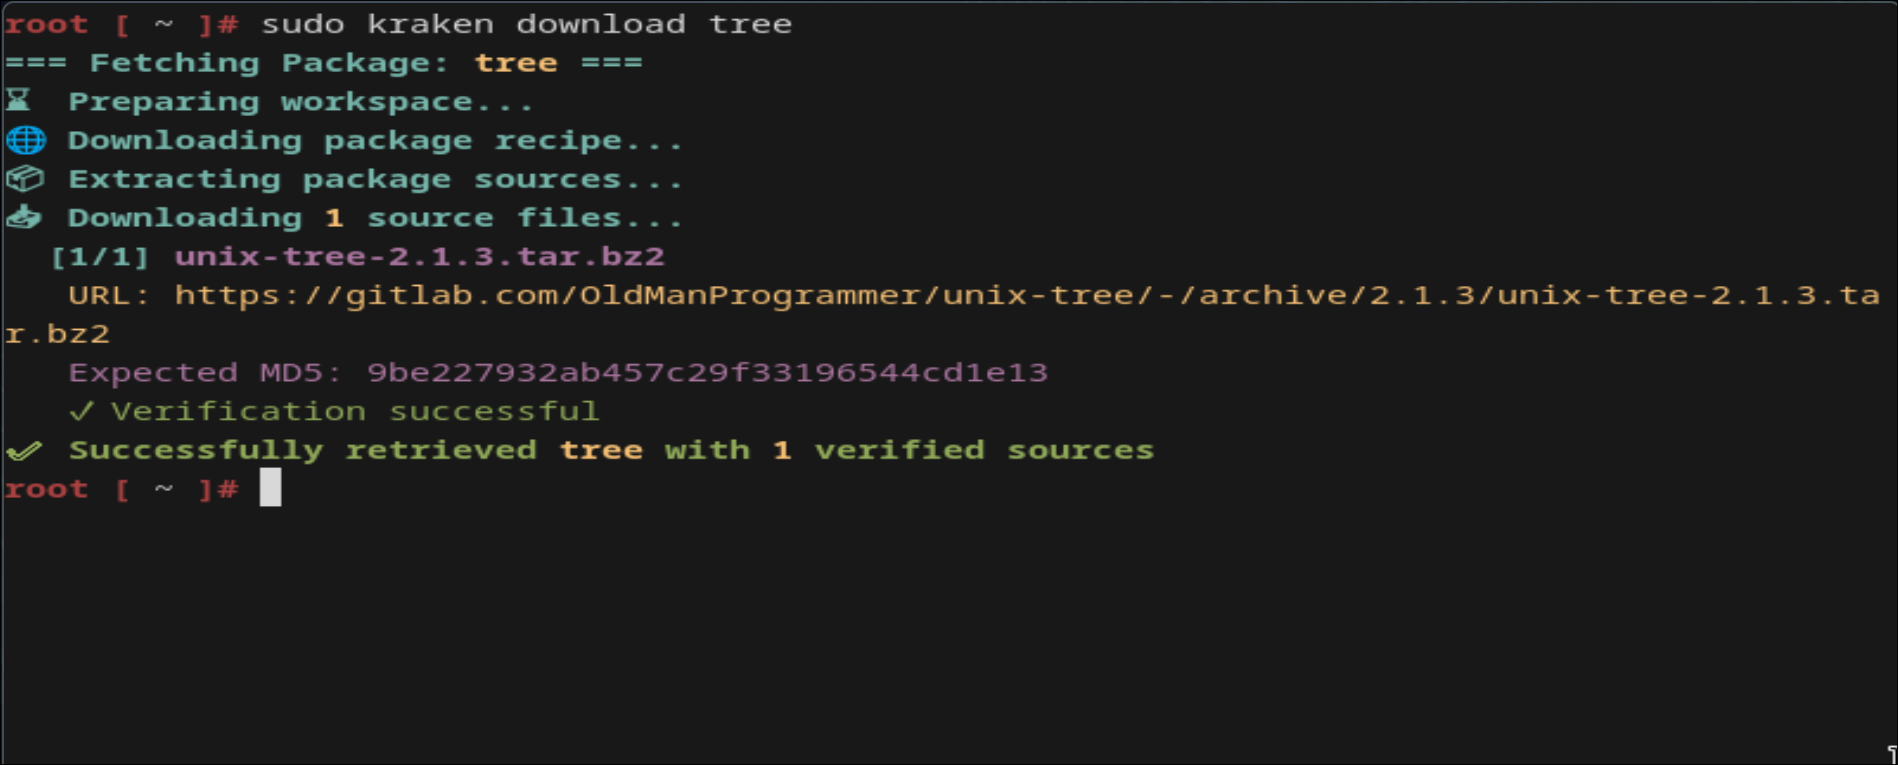
\includegraphics[width=1\textwidth, height=10cm]{images_pfe/downlad.png}
  %\caption{Exemple pratique de l’outil \texttt{kraken download}}
  %\label{fig:pkgtemplate}
%\end{figure}




\subsection{kraken prepare}

\textbf{Utilisation :} \texttt{sudo kraken prepare <nom\_du\_paquet>}

Cet outil est conçu pour préparer le paquet avant sa compilation.

\paragraph{Étapes de fonctionnement :}
\begin{enumerate}
    \item Interroger la base de données pour vérifier si le paquet a été téléchargé.
    \item Si oui, localiser l’archive et l’extraire (en utilisant \texttt{tar}, \texttt{unzip}, etc., selon le format).
    \item Extraire la fonction \texttt{kraken\_prepare()} du fichier \texttt{PKGBUILD.kraken} du paquet, et l’exécuter.
    \item Mettre à jour la base de données en marquant le paquet comme préparé (\texttt{prepared = 1}).
\end{enumerate}

%\begin{figure}[H]
 % \centering
  %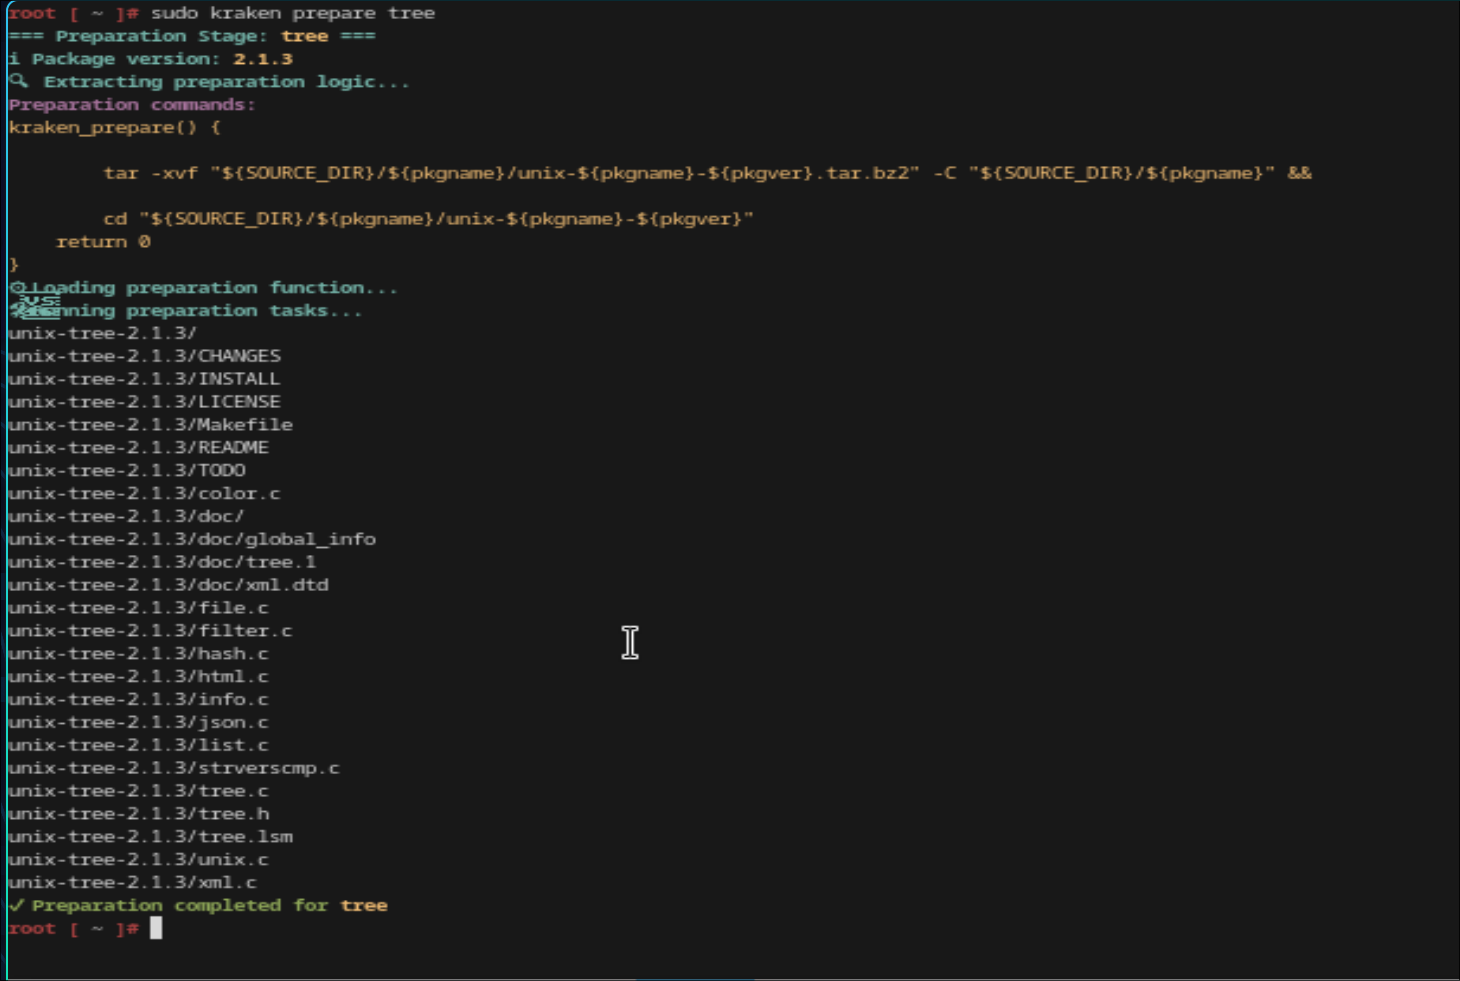
\includegraphics[width=1\textwidth, height=10cm]{images_pfe/prepare.png}
  %\caption{Exemple pratique de l’outil \texttt{kraken prepare}}
  %\label{fig:pkgtemplate}
%\end{figure}





\subsection{kraken build}

\textbf{Utilisation :} \texttt{sudo kraken build <nom\_du\_paquet>}

Cet outil est conçu pour compiler les paquets à l’aide de leur système de build (\texttt{make}, \texttt{ninja}, \texttt{meson}, etc.).

\paragraph{Étapes de fonctionnement :}
\begin{enumerate}
    \item Interroger la base de données pour vérifier si le paquet a été préparé.
    \item Si oui,  Extraire la fonction \texttt{build()} du fichier \texttt{PKGBUILD.kraken} et l’exécuter pour compiler le paquet (génération de bibliothèques, binaires, etc.).
    \item Mettre à jour la base de données en marquant le paquet comme compilé (\texttt{built = 1}).
\end{enumerate}







\subsection{kraken test}

\textbf{Utilisation :} \texttt{sudo kraken test <nom\_du\_paquet>}

\paragraph{Étapes de fonctionnement :}
\begin{enumerate}
    \item Interroger la base de données pour vérifier si le paquet a été compilé.
    \item Si oui, Extraire la fonction \texttt{test()} depuis le fichier \texttt{PKGBUILD.kraken}, et l’exécuter afin de tester le paquet compilé.
\end{enumerate}

\textbf{Remarque :} les tests sont optionnels. Certains paquets ne fournissent pas de suite de test officielle, donc l'exécution de cette étape n'est pas considérée comme critique.

%\begin{figure}[H]
 % \centering
 % 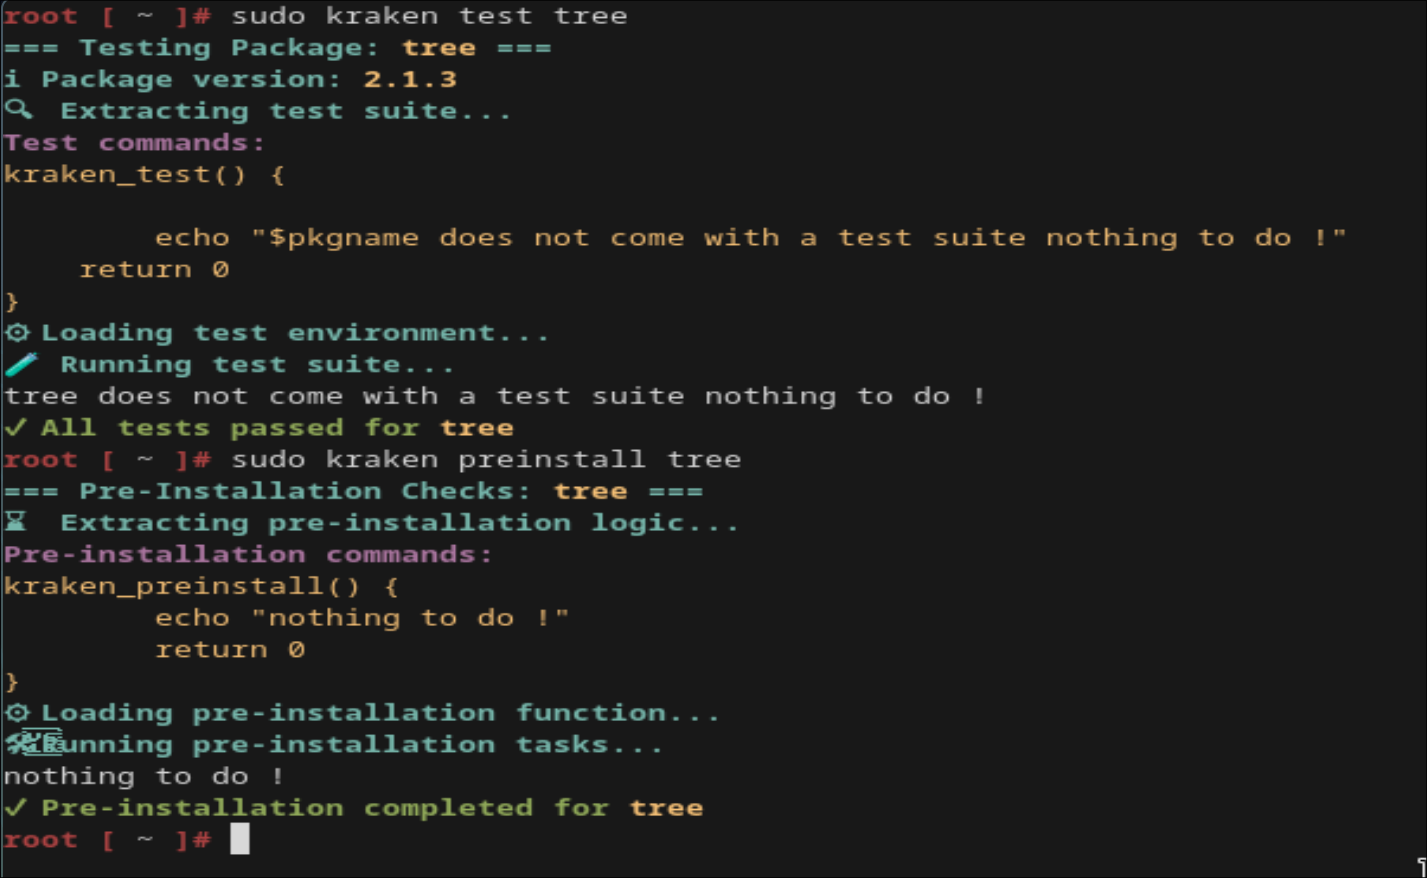
\includegraphics[width=1\textwidth, height=10cm]{images_pfe/test.png}
 % \caption{Exemple pratique de l’outil \texttt{kraken test}}
 % \label{fig:pkgtemplate}
%\end{figure}










\subsection*{Principe de la « fausse installation »}  
\label{subsecc:fakeinstall}
Comme nous l'avons vu dans le chapitre \ref{subsec:suivi-fichiers}, nous devons implémenter un mécanisme qui installe les paquets de manière fictive dans un répertoire temporaire afin de détecter tous les fichiers et répertoires créés par le paquet lors de l'installation. Cette étape sera utilisée ultérieurement dans le mécanisme de suppression des paquets.

\textbf{Utilisation :} \texttt{sudo kraken fakeinstall <nom\_du\_paquet>}

\textbf{Étapes :}
\begin{enumerate}
  \item Vérifier si le paquet a été compiler  ou non à partir de la base de données.
  \item Si oui, Extraire la fonction \texttt{kraken-install} du fichier \texttt{pkgbuild.kraken} et créer un répertoire temporaire situé dans \texttt{/tmp} où le paquet sera installé \textbf{fictivement}, en forçant l’installation dans ce répertoire de destination.
  \item Créer un environnement fictif à l’aide de l’outil \textbf{fakeroot}.
  \item Lancer l’installation du paquet  en parallèle avec l’outil \textbf{strace} afin de détecter tous les changements effectués sur le système.
  \item Générer les métadonnées dans :
  \begin{itemize}
    \item \texttt{/var/lib/kraken/packages/DIRS} -- contient tous les répertoires marqués par le paquet.
    \item \texttt{/var/lib/kraken/packages/FILES} -- contient tous les fichiers marqués par le paquet.
  \end{itemize}
\end{enumerate}

%La figure suivante montre un exemple pratique de l'utilisation de l’outil \texttt{fakeinstall} :

%\begin{figure}[H]
%  \centering
 % 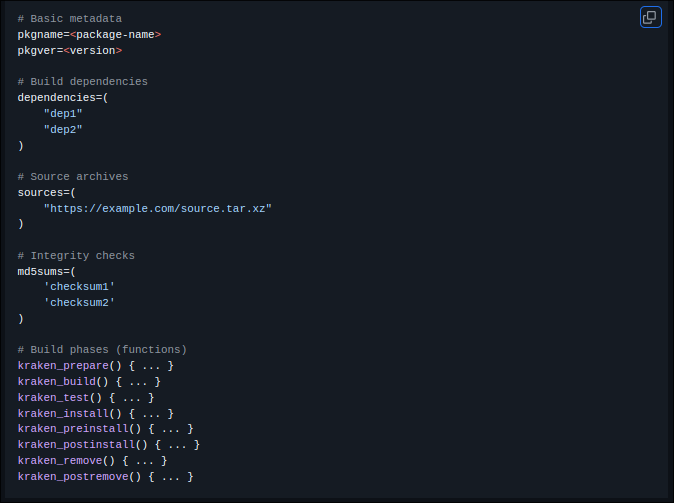
\includegraphics[width=1\textwidth, height=10cm]{images_pfe/pkgbuildkrakenmodle.png}
  %\caption{Modèle de fichier \texttt{pkgbuild.kraken}}
  %\label{fig:pkgtemplate}
%\end{figure}


%\textcolor{red}{Cette figure illustre un exemple des fichiers et répertoires de métadonnées générés pour un paquet (\texttt{DIRS} et %\texttt{FILES}) :}

%\begin{figure}[H]
%  \centering
%  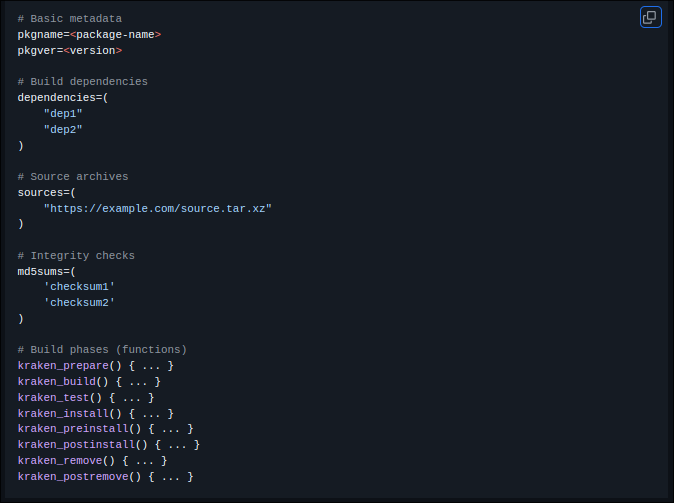
\includegraphics[width=1\textwidth, height=10cm]{images_pfe/pkgbuildkrakenmodle.png}
%  \caption{Modèle de fichier \texttt{pkgbuild.kraken}}
%  \label{fig:pkgtemplate}
%\end{figure}

%\textbf{Remarque :} Comme vous pouvez le voir dans la figure, les fichiers \texttt{DIRS} et \texttt{FILES} contiennent certains répertoires %critiques tels que \texttt{/usr}, \texttt{/boot}, \texttt{/bin}, \texttt{/root}. Il est donc nécessaire de mettre en place un mécanisme de %filtrage de ces répertoires afin de garantir que le système de fichiers critique ne soit pas altéré lors de la suppression d’un paquet.





\subsection{kraken install}

\textbf{Utilisation :} \texttt{sudo kraken install <nom\_du\_paquet>}

Cet outil est conçu pour installer les paquets dans le système final.

\textbf{Étapes :}
\begin{enumerate}
  \item Vérifier si le paquet a été installé fictivement (fakeinstall) dans la base de données.
  \item Si oui, Exécuter la fonction \texttt{install} située dans le fichier \texttt{pkgbuild.kraken}.
  \item Marquer le paquet comme installé définitivement dans le système avec la date d’installation.
\end{enumerate}



%\begin{figure}[H]
%  \centering
%  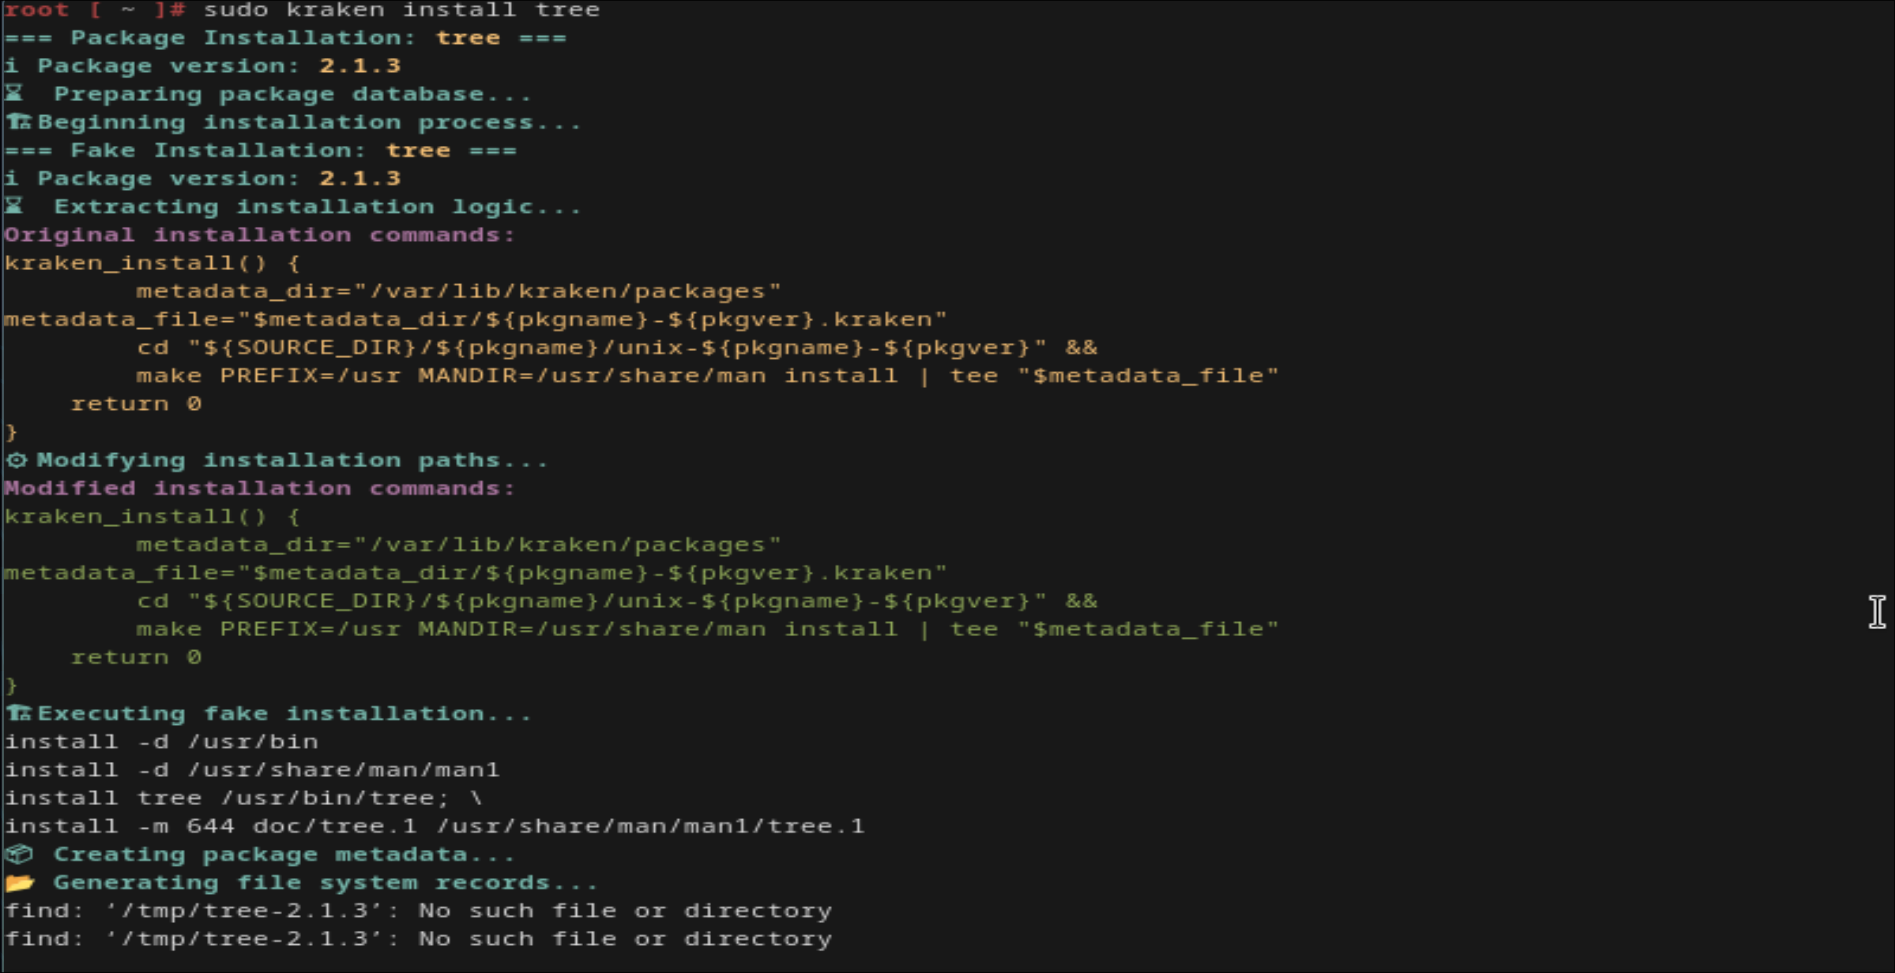
\includegraphics[width=1\textwidth, height=10cm]{images_pfe/install.png}
%  \caption{Modèle de fichier \texttt{pkgbuild.kraken}}
%  \label{fig:pkgtemplate}
%\end{figure}





\subsection{kraken postinstall}

\textbf{Utilisation :} \texttt{sudo kraken postinstall <nom\_du\_paquet>}

Cet outil est conçu pour exécuter les configurations post-installation après l’installation du paquet, comme la modification de certains fichiers de configuration.

\textbf{Étapes :}
\begin{enumerate}
  \item Vérifier si le paquet est installé dans le système en consultant la base de données.
  \item Si oui, Exécuter la fonction \texttt{postinstall} à partir du fichier \texttt{pkgbuild.kraken}.
\end{enumerate}

%La figure suivante montre un exemple d’utilisation de l’outil \texttt{postinstall} :

%\begin{figure}[H]
%  \centering
 % 
\includegraphics[width=1\textwidth, height=10cm]{images_pfe/alpine.jpg}
 % \caption{Modèle de fichier \texttt{pkgbuild.kraken}}
 % \label{fig:pkgtemplate}
%\end{figure}
%\textcolor{blue}{Pour voir une vidéo de démonstration de l’utilisation de ces outils pour installer un paquet, voir \cite{kraken_tools}.}

\subsection{kraken remove}

\textbf{Utilisation :} \texttt{sudo kraken remove <nom\_du\_paquet>}

Ce mécanisme prend en charge deux cas :

\begin{enumerate}
  \item Détecter si le paquet possède un mécanisme de désinstallation dans son système de construction. Si oui, nous l’utilisons pour supprimer le paquet.
  \item Si le paquet ne possède pas de mécanisme de désinstallation, nous appelons un mécanisme nommé \texttt{manual\_install}. Celui-ci parcourt les fichiers de métadonnées (\texttt{FILES}, \texttt{DIRS}) créés lors de l’étape \texttt{fakeinstall}, et supprime tous les fichiers et répertoires listés.
  \item Mettre à jour la base de données en supprimant le paquet de la table des paquets installés.
\end{enumerate}



%\begin{figure}[H]
 % \centering
  %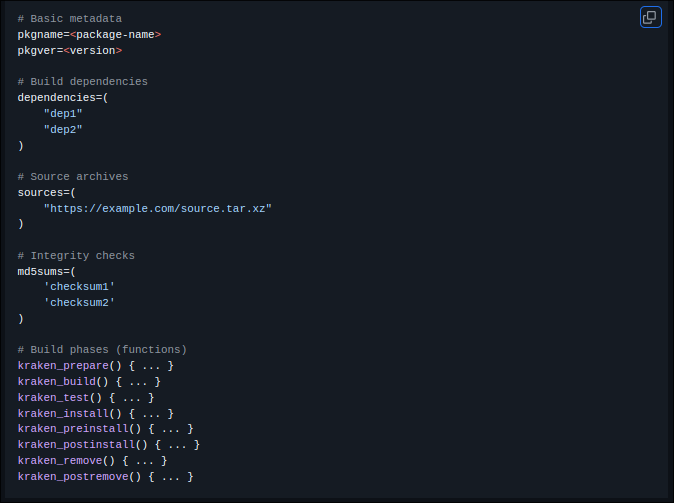
\includegraphics[width=1\textwidth, height=10cm]{images_pfe/pkgbuildkrakenmodle.png}
  %\caption{Modèle de fichier \texttt{pkgbuild.kraken}}
  %\label{fig:pkgtemplate}
%\end{figure}

\subsection{kraken entropy}

\textbf{Utilisation :} \texttt{sudo kraken entropy <nom\_du\_paquet>}

Cet outil est conçu pour installer \textbf{automatiquement} le paquet ainsi que toutes ses dépendances.

\textbf{Étapes :}
\begin{enumerate}
  \item Construire le graphe complet du paquet, affichant toutes les dépendances et les dépendances des dépendances.
  \item Détecter s'il y a des cycles dans le graphe ou des dépendances de type config ou diamant. Pour en savoir plus sur ces problèmes, référez-vous au section \textcolor{blue}{\ref{subsec:circular-dependencies}}.
  \item Parcourir le graphe en utilisant la recherche en profondeur (Depth First Search) et installer chaque paquet dans le bon ordre en utilisant les outils précédents (\texttt{download}, \texttt{prepare}, \texttt{build}, \texttt{test}, \texttt{fakeinstall}, \texttt{install}, \texttt{postinstall}).
\end{enumerate}

%Exemple illustrant le mécanisme d'entropie :

%\begin{figure}[H]
 % \centering
 % 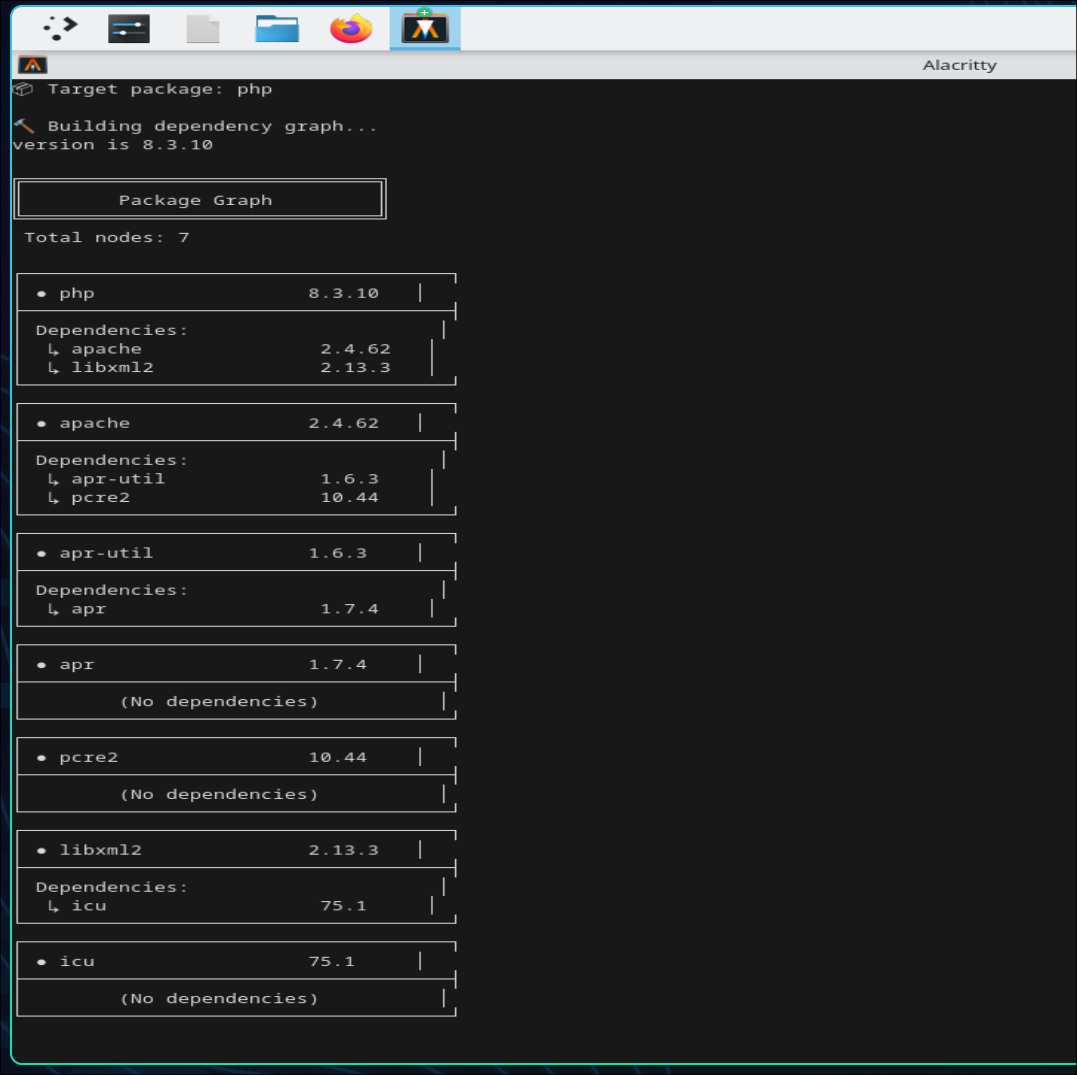
\includegraphics[width=1\textwidth, height=13cm]{images_pfe/phpgraph.png}
 % \caption{Modèle de fichier \texttt{pkgbuild.kraken}}
 % \label{fig:pkgtemplate}
%\end{figure}


\subsection{kraken getversion}

\textbf{Utilisation :} \texttt{sudo kraken getversion <nom\_du\_paquet>}

Cet outil est conçu pour afficher la version d'un paquet, qu'il soit installé ou non ( depuis le dépôt).


\subsection{kraken dependency}

\textbf{Utilisation :} \texttt{sudo kraken getdeps <nom\_du\_paquet> <version\_du\_paquet>}

Généralement, si vous choisissez de construire le paquet manuellement, vous devez vérifier ses dépendances. Cet outil affiche les dépendances d'un paquet en utilisant \texttt{yq} pour interroger le \texttt{pkgindex.kraken}.



\subsection{kraken checkinstaller}

\textbf{Utilisation :} \texttt{sudo kraken checkinstalled <nom\_du\_paquet>}

Cet outil détecte si le paquet est installé dans le système ou non en interrogeant la base de données.

 
\subsection{Outils en développement}

Comme vous pouvez le voir, notre gestionnaire de paquets construit le paquet à partir des sources, mais nous prévoyons d'améliorer cette fonctionnalité dans les futures versions. Nous préparons le développement d'un mécanisme pour :\\

  permettant de compiler le paquet à l'intérieur de Kraken OS, hébergé dans une machine virtuelle sur un serveur cloud. L'idée est de générer un nouveau tarball \textbf{reconstruit} nommé \texttt{pkgnam-pkgversion.kraken}.\\
Ce tarball sera compilé et configuré dans le cloud, et l'utilisateur n'aura qu'à l'installer sur son système sans avoir à le compiler lui-même.
Cela permettra de réduire le temps de compilation, car la construction de paquets à partir des sources est fastidieuse et consomme beaucoup de ressources et de temps. Par exemple, compiler un paquet comme \texttt{gcc} peut prendre 4 heures avec 6 cœurs.\\

\bigbreak

\textcolor{blue}{Code source  de notre gestionnaires de paquetes kraken  disponible dans  \cite{gestionnaire_paquets}}.\\
\bigbreak
\textcolor{blue}{Pour voir une vidéo de démonstration de l’utilisation de ces outils pour installer un paquet manuellement, voir \cite{kraken_tools}.}\\
\bigbreak
\textcolor{blue}{Pour voir une vidéo de démonstration de l’utilisation de loutil, \texttt{kraken-entropy}, pour installer \textbf{automatiquement} un paquet avec \textbf{la résolution de ses dépendances}, voir \cite{kraken_entropy}.}\\
\bigbreak
\section{Conclusion}
Notre distribution atteint désormais un stade fonctionnel complet, incluant un gestionnaire de paquets \textbf{basique}.\\
La prochaine phase  produire une ISO installable pour permettre son déploiement massif.